% Options for packages loaded elsewhere
\PassOptionsToPackage{unicode}{hyperref}
\PassOptionsToPackage{hyphens}{url}
\PassOptionsToPackage{dvipsnames,svgnames,x11names}{xcolor}
%
\documentclass[
]{article}
\usepackage{amsmath,amssymb}
\usepackage{iftex}
\ifPDFTeX
  \usepackage[T1]{fontenc}
  \usepackage[utf8]{inputenc}
  \usepackage{textcomp} % provide euro and other symbols
\else % if luatex or xetex
  \usepackage{unicode-math} % this also loads fontspec
  \defaultfontfeatures{Scale=MatchLowercase}
  \defaultfontfeatures[\rmfamily]{Ligatures=TeX,Scale=1}
\fi
\usepackage{lmodern}
\ifPDFTeX\else
  % xetex/luatex font selection
\fi
% Use upquote if available, for straight quotes in verbatim environments
\IfFileExists{upquote.sty}{\usepackage{upquote}}{}
\IfFileExists{microtype.sty}{% use microtype if available
  \usepackage[]{microtype}
  \UseMicrotypeSet[protrusion]{basicmath} % disable protrusion for tt fonts
}{}
\makeatletter
\@ifundefined{KOMAClassName}{% if non-KOMA class
  \IfFileExists{parskip.sty}{%
    \usepackage{parskip}
  }{% else
    \setlength{\parindent}{0pt}
    \setlength{\parskip}{6pt plus 2pt minus 1pt}}
}{% if KOMA class
  \KOMAoptions{parskip=half}}
\makeatother
\usepackage{xcolor}
\usepackage[margin=1in]{geometry}
\usepackage{longtable,booktabs,array}
\usepackage{calc} % for calculating minipage widths
% Correct order of tables after \paragraph or \subparagraph
\usepackage{etoolbox}
\makeatletter
\patchcmd\longtable{\par}{\if@noskipsec\mbox{}\fi\par}{}{}
\makeatother
% Allow footnotes in longtable head/foot
\IfFileExists{footnotehyper.sty}{\usepackage{footnotehyper}}{\usepackage{footnote}}
\makesavenoteenv{longtable}
\usepackage{graphicx}
\makeatletter
\def\maxwidth{\ifdim\Gin@nat@width>\linewidth\linewidth\else\Gin@nat@width\fi}
\def\maxheight{\ifdim\Gin@nat@height>\textheight\textheight\else\Gin@nat@height\fi}
\makeatother
% Scale images if necessary, so that they will not overflow the page
% margins by default, and it is still possible to overwrite the defaults
% using explicit options in \includegraphics[width, height, ...]{}
\setkeys{Gin}{width=\maxwidth,height=\maxheight,keepaspectratio}
% Set default figure placement to htbp
\makeatletter
\def\fps@figure{htbp}
\makeatother
\setlength{\emergencystretch}{3em} % prevent overfull lines
\providecommand{\tightlist}{%
  \setlength{\itemsep}{0pt}\setlength{\parskip}{0pt}}
\setcounter{secnumdepth}{5}
\newlength{\cslhangindent}
\setlength{\cslhangindent}{1.5em}
\newlength{\csllabelwidth}
\setlength{\csllabelwidth}{3em}
\newlength{\cslentryspacingunit} % times entry-spacing
\setlength{\cslentryspacingunit}{\parskip}
\newenvironment{CSLReferences}[2] % #1 hanging-ident, #2 entry spacing
 {% don't indent paragraphs
  \setlength{\parindent}{0pt}
  % turn on hanging indent if param 1 is 1
  \ifodd #1
  \let\oldpar\par
  \def\par{\hangindent=\cslhangindent\oldpar}
  \fi
  % set entry spacing
  \setlength{\parskip}{#2\cslentryspacingunit}
 }%
 {}
\usepackage{calc}
\newcommand{\CSLBlock}[1]{#1\hfill\break}
\newcommand{\CSLLeftMargin}[1]{\parbox[t]{\csllabelwidth}{#1}}
\newcommand{\CSLRightInline}[1]{\parbox[t]{\linewidth - \csllabelwidth}{#1}\break}
\newcommand{\CSLIndent}[1]{\hspace{\cslhangindent}#1}
\usepackage{caption}
\usepackage{booktabs}
\usepackage{longtable}
\usepackage{array}
\usepackage{multirow}
\usepackage{wrapfig}
\usepackage{float}
\usepackage{colortbl}
\usepackage{pdflscape}
\usepackage{tabu}
\usepackage{threeparttable}
\usepackage{threeparttablex}
\usepackage[normalem]{ulem}
\usepackage{makecell}
\usepackage{xcolor}
\ifLuaTeX
  \usepackage{selnolig}  % disable illegal ligatures
\fi
\IfFileExists{bookmark.sty}{\usepackage{bookmark}}{\usepackage{hyperref}}
\IfFileExists{xurl.sty}{\usepackage{xurl}}{} % add URL line breaks if available
\urlstyle{same}
\hypersetup{
  pdftitle={Binocular combination in the autonomic nervous system},
  colorlinks=true,
  linkcolor={black},
  filecolor={Maroon},
  citecolor={Blue},
  urlcolor={Blue},
  pdfcreator={LaTeX via pandoc}}

\title{Binocular combination in the autonomic nervous system}
\author{Federico G. Segala\(^1\), Joel T. Martin\(^1\), Annie Y. Morsi\(^1\), Alex R. Wade\(^{1,2}\) \& Daniel H. Baker\(^{1,2}\)}
\date{}

\begin{document}
\maketitle

\(^1\)Department of Psychology, University of York, Heslington, York, United Kingdom.

\(^2\)York Biomedical Research Institute, University of York, Heslington, York, United Kingdom.

Address for correspondence: Federico G. Segala, \url{federico.segala@york.ac.uk}

\hypertarget{abstract-250-words}{%
\section{Abstract (250 words)}\label{abstract-250-words}}

The diameter of the pupil fluctuates in response to levels of ambient light and is regulated by the autonomic nervous system. Increasing light in one eye causes both pupils to constrict, implying the system must combine signals across the two eyes, a process of binocular integration occuring independently of visual cortex. Distinct classes of retinal photoreceptor are involved in controlling and maintaining pupil diameter, with cones and rods driving the initial constriction and intrinsically photosensitive retinal ganglion cells maintaining diameter over prolonged time periods. Here, we used silent substitution to investigate binocular combination while targeting different photoreceptor pathways with sinusoidally modulated inputs. We find different patterns of binocular response in each pathway, and across the first and second harmonic frequencies. At the first harmonic, luminance and S-cone responses showed strong binocular facilitation, and weak interocular suppression. Melanopsin responses were invariant to the number of eyes stimulated. Notably, the L-M pathway involved binocular inhibition, whereby responses to binocular stimulation were weaker than for monocular stimulation. The second harmonic involved greater binocular facilitation in all pathways, and we show that binocular facilitation is negatively correlated with the magnitude of dichoptic masking. Our results are consistent with a computational model of binocular signal combination (implemented in a Bayesian hierarchical framework), in which the weight of interocular suppression differs across pathways. We also find pathway differences in response phase, consistent with different lag times for phototransduction. This work demonstrates for the first time the algorithm governing binocular combination in the autonomic nervous system.

\hypertarget{significance-statement-120-words}{%
\section{Significance statement (120 words)}\label{significance-statement-120-words}}

\hypertarget{introduction}{%
\section{Introduction}\label{introduction}}

The autonomic nervous system regulates many involuntary bodily processes, including the constriction and dilation of the pupils in response to light (\protect\hyperlink{ref-McDougal2015}{McDougal and Gamlin, 2015}). The anatomical pathway from the retina to the subcortical nuclei controlling the pupillary light response (PLR) is well established: it includes the Pretectal Olivary nucleus (PON), the Superior Cervical ganglion and the Edinger-Westphal nucleus, which project to the iris sphincter muscles that directly control the pupil size (\protect\hyperlink{ref-McDougal2015}{McDougal and Gamlin, 2015}, \protect\hyperlink{ref-McDougal2008}{2008}; \protect\hyperlink{ref-Wang2015}{Wang and Munoz, 2015}). Evidence of a binocular component to the PLR is shown by the existence of a consensual response of the pupil (the stimulation of one eye will cause constriction of the other eye, \protect\hyperlink{ref-Wyatt1981}{Wyatt and Musselman, 1981}). The anatomical segregation of the subcortical pathway from the rest of the brain means that this binocular combination of signals must occur independently of the cortical processes of binocular integration required for visual perception. Our recent work (\protect\hyperlink{ref-Segala2023}{Segala et al., 2023}) has shown that the algorithm underlying binocular combination of light in the pupil pathway differs from that in the cortex. Here we extend this paradigm to compare binocular combination in different photoreceptor pathways that feed into the autonomic nervous system.

Different classes of retinal photoreceptors, including cones, rods and the recently discovered melanopsin-containing intrinsically photosensitive retinal ganglion cells (ipRGCs), are directly involved in controlling and maintaining the size of the pupils (\protect\hyperlink{ref-Barrionuevo2018}{Barrionuevo et al., 2018}; \protect\hyperlink{ref-Barrionuevo2014}{Barrionuevo et al., 2014}; \protect\hyperlink{ref-Dacey2005}{Dacey et al., 2005}; \protect\hyperlink{ref-Murray2018}{Murray et al., 2018}; \protect\hyperlink{ref-Spitschan2019}{Spitschan, 2019}; \protect\hyperlink{ref-Spitschan2014}{Spitschan et al., 2014}; \protect\hyperlink{ref-Woelders2018}{Woelders et al., 2018}). The cones have been shown to drive the initial rapid constriction of the pupils (\protect\hyperlink{ref-Mathot2018}{Mathôt, 2018}), while the slower and longer activation of the ipRGCs shows their role in maintaining the constriction over a prolonged period of time and in regulating the post-illumination pupillary response (\protect\hyperlink{ref-Markwell2010}{Markwell et al., 2010}; \protect\hyperlink{ref-McDougal2010}{McDougal and Gamlin, 2010}). The ipRGCs are a unique photoreceptor class that has been discovered recently (\protect\hyperlink{ref-Provencio2000}{Provencio et al., 2000}). They express the photopigment melanopsin, and are involved in the regulation of the circadian rhythm (\protect\hyperlink{ref-Panda2002}{Panda et al., 2002}; \protect\hyperlink{ref-Provencio2000}{Provencio et al., 2000}; \protect\hyperlink{ref-Ruby2002}{Ruby et al., 2002}), forming a major input to the PON (\protect\hyperlink{ref-Dacey2003}{Dacey et al., 2003}). The first direct evidence of the involvement of the ipRGCs in the PLR was shown in rats by Lucas et al. (\protect\hyperlink{ref-Lucas2003}{2003}) who genetically deleted the melanopsin gene from rats, resulting in the loss of the intrinsic photosensitivity of the cells and a reduced pupil constriction. This same behaviour was later also observed in primates and humans (\protect\hyperlink{ref-Gamlin2007}{Gamlin et al., 2007}), where it was demonstrated that the PLR continues during light presentation even when cone and rod signalling is blocked, indicating the primary role of the ipRGCs in maintaining pupil constriction over a prolonged time.

A technique known as silent substitution (\protect\hyperlink{ref-Estevez1982}{Estévez and Spekreijse, 1982}) can be used to selectively stimulate specific photoreceptor classes. Silent substitution exploits the fact that each photoreceptor class has a distinct spectral tuning that overlaps with the others. Using a multiprimary system, in which the primaries have different spectra, it is possible to target one class of photoreceptors while maintaining the others at a constant activity level, effectively silencing them (\protect\hyperlink{ref-Shapiro1996}{Shapiro et al., 1996}; \protect\hyperlink{ref-Spitschan2018}{Spitschan and Woelders, 2018}, this paper also offers a clear explanation of how to implement silent substitution). Studies using silent substitution have shown that the pupils behave differently depending on which photoreceptor or pathway is being stimulated. For example, pupil responses have been shown to be out of phase when the S cones are stimulated, relative to when the ipRGCs or the L+M cones are stimulated (\protect\hyperlink{ref-Cao2015}{Cao et al., 2015}; \protect\hyperlink{ref-Spitschan2014}{Spitschan et al., 2014}). Additionally, when L and M cones are stimulated individually, there appears to be a paradoxical pupil response: increments in L cone stimulation cause a constriction of the pupil, while increments in M cone stimulation lead to a dilation of the pupil (\protect\hyperlink{ref-Murray2018}{Murray et al., 2018}; \protect\hyperlink{ref-Woelders2018}{Woelders et al., 2018}).

Binocular combination has been extensively studied in visual perception, where it is mediated by neurons in primary visual cortex (\protect\hyperlink{ref-Hubel1962}{Hubel and Wiesel, 1962}; \protect\hyperlink{ref-Moradi2009}{Moradi and Heeger, 2009}). For pattern vision, binocular summation occurs at threshold, such that less contrast is required to detect a target shown to both eyes than for a target shown to only one eye (\protect\hyperlink{ref-Baker2018}{Baker et al., 2018}; \protect\hyperlink{ref-Campbell1965}{Campbell and Green, 1965}; \protect\hyperlink{ref-Legge1984}{Legge, 1984}). At higher contrasts, a process of `ocularity invariance' is observed, in which the response to monocularly- and binocularly-presented patterns is equal (\protect\hyperlink{ref-Baker2007}{Baker et al., 2007}; \protect\hyperlink{ref-Ding2006}{Ding and Sperling, 2006}; \protect\hyperlink{ref-Meese2006}{Meese et al., 2006}; \protect\hyperlink{ref-Moradi2009}{Moradi and Heeger, 2009}). This is thought to be due to a process of interocular suppression that compensates for the additional excitatory drive caused by stimulating two eyes. Our recent work (\protect\hyperlink{ref-Segala2023}{Segala et al., 2023}) has shown that cortical signal combination for luminance flicker is substantially more linear than for spatial patterns, whereas there is evidence of interocular suppression in the pupil pathway.

Most studies that use silent substitution to investigate the PLR stimulate only one eye. If the stimulated eye is pharmacologically dilated to control pupil size, the response from the unstimulated eye (known as the consensual response) can be recorded (e.g. \protect\hyperlink{ref-McDougal2010}{McDougal and Gamlin, 2010}; \protect\hyperlink{ref-Spitschan2014}{Spitschan et al., 2014}). While this approach controls the total amount of light incident at the retina, it does not permit investigation of binocular combination for specific photoreceptor pathways. Here we take a different approach, using a custom binocular multiprimary system (see Figure \ref{fig:spectraplots}a,b) that can modulate each (undilated) eye independently, and a binocular eye tracker to measure the diameter of both pupils. We measure the amplitude of pupil modulation (using Fourier analysis) in response to sinusoidal stimulation at 0.5Hz, for stimuli directed at the luminnce pathway, L-M cone pathway, S-cone pathway, and melanopsin pathway. Our key comparisons are between monocular and binocular stimulation, and between monocular stimulation and a dichoptic masking condition in which the non-target eye is stimulated by a high contrast mask signal at a different frequency (0.4Hz). The results are interpreted using a contemporary model of binocular vision (\protect\hyperlink{ref-Meese2006}{Meese et al., 2006}) implemented within a hierarchical Bayesian framework

\hypertarget{results}{%
\section{Results}\label{results}}

Figure \ref{fig:spectraplots}m-p shows averaged waveforms of pupil diameter in response to binocular stimulation. For luminance stimuli (Figure \ref{fig:spectraplots}m) a strong modulation is apparent at the stimulation frequency (0.5Hz), which is also clear in the Fourier amplitude spectrum (Figure \ref{fig:spectraplots}q). For binocular stimulation of the L-M pathway, S-cone pathway and melanopsin pathway, pupil modulations were less than 10\% of the amplitude of the luminance modulation (note the change in y-axis scale for the Fourier spectra), but still apparent at 0.5Hz in the Fourier spectra (Figure \ref{fig:spectraplots}n-p). We also observed a second harmonic response (at 1Hz) for all conditions, which was weaker than the first harmonic for luminance and melanopsin stimulation, but stronger for L-M and S-cone stimulation. The additional component is also apparent in the pupil waveforms shown in Figure \ref{fig:spectraplots}n-p.~Our main analysis therefore focuses on the amplitude of the pupil modulations at both the first and second harmonic frequencies across different stimulus conditions.

\begin{figure}

{\centering 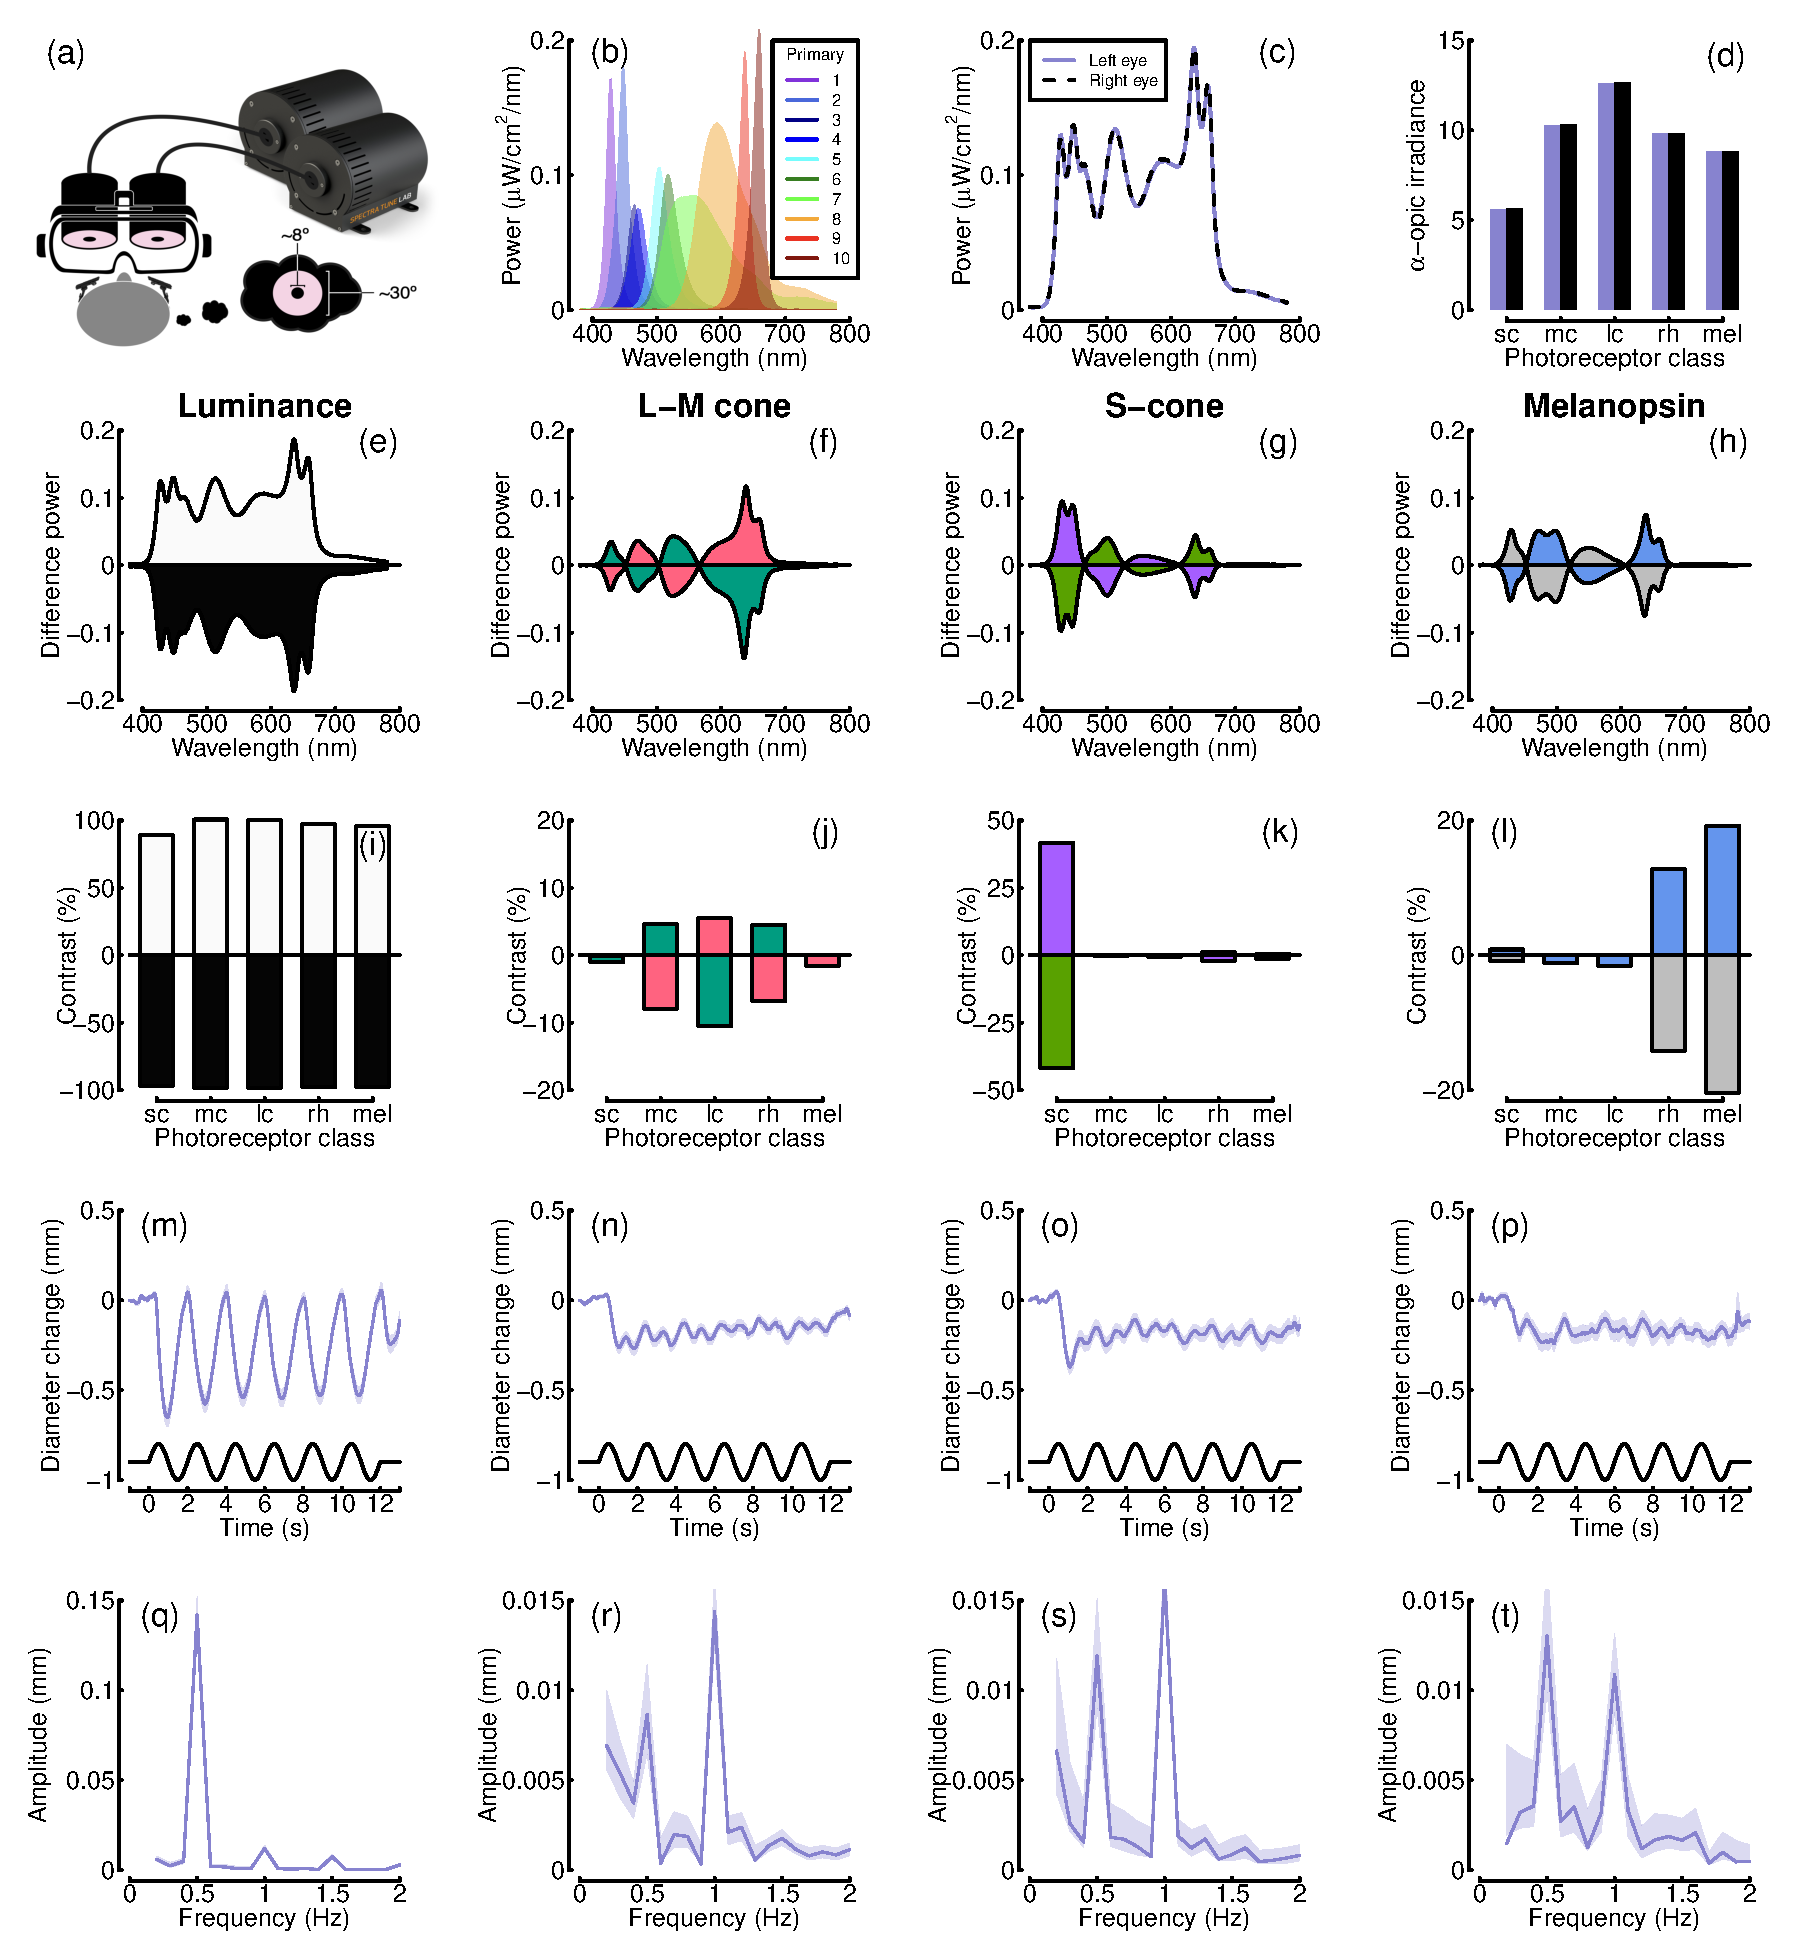
\includegraphics[width=0.8\linewidth]{Figures/methodsfig} 

}

\caption{Summary of the spectral power distributions and alpha-opic irradiances for the background and each condition, as well as averaged pupil diameters and Fourier spectra. Panel (a) shows a schematic of the binocular stimulation system for presenting spectrally tuned modulations independently to each eye. The VR headset was attached to a clamp stand that the experimenters could use to adjust the height and align the headset with the eyes of the participant. The participant's head was supported by a chin rest to keep it in position throughout the experiment. Panel (b) shows the outputs of each LED primary at maximum intensity, and panels (c) and (d) show the overall spectral power distributions and the alpha-opic irradiances of the background spectra used for both eyes. The subsequent rows show the power differences (e-h), and alpha-opic irradiances (i-l) relative to the background, averaged pupil diameter waveform (m-p) and Fourier spectra (q-t) for binocular stimulation. Column headings indicate the pathway stimulated, and shaded regions in panels m-t indicate bootstrapped 95\% confidence intervals.}\label{fig:spectraplots}
\end{figure}

Figure \ref{fig:CRFplots} shows contrast response functions across stimulation conditions for responses at the first harmonic (panels a-d) and the second harmonic (panels e-h) frequencies. In each plot, the response to monocular stimulation is given by the red circles and typically increases monotonically as a function of stimulus (temporal) contrast (main effects of stimulus contrast are significant for all data sets, see Supplementary Materials). Relative to monocular stimulation, binocular stimulation typically led to higher response amplitudes, indicating a binocular facilitation effect (main effects of condition are significant for all data sets, see Supplementary Materials). This is strongest for the luminance and S-cone conditions at the first harmonic (Figure \ref{fig:CRFplots}a,c) and the L-M cone and Melanopsin conditions at the second harmonic (Figure \ref{fig:CRFplots}f,h). One striking exception to this pattern is in the L-M cone condition at the first harmonic (Figure \ref{fig:CRFplots}b): this condition produced a binocular suppression effect, where the response to binocular stimulation is weaker than the response to monocular stimulation (blue squares below red circles). These results indicate that the magnitude of binocular facilitation differs across photoreceptor pathway, suggesting heterogeneity in the underlying neural computation.

\begin{figure}

{\centering 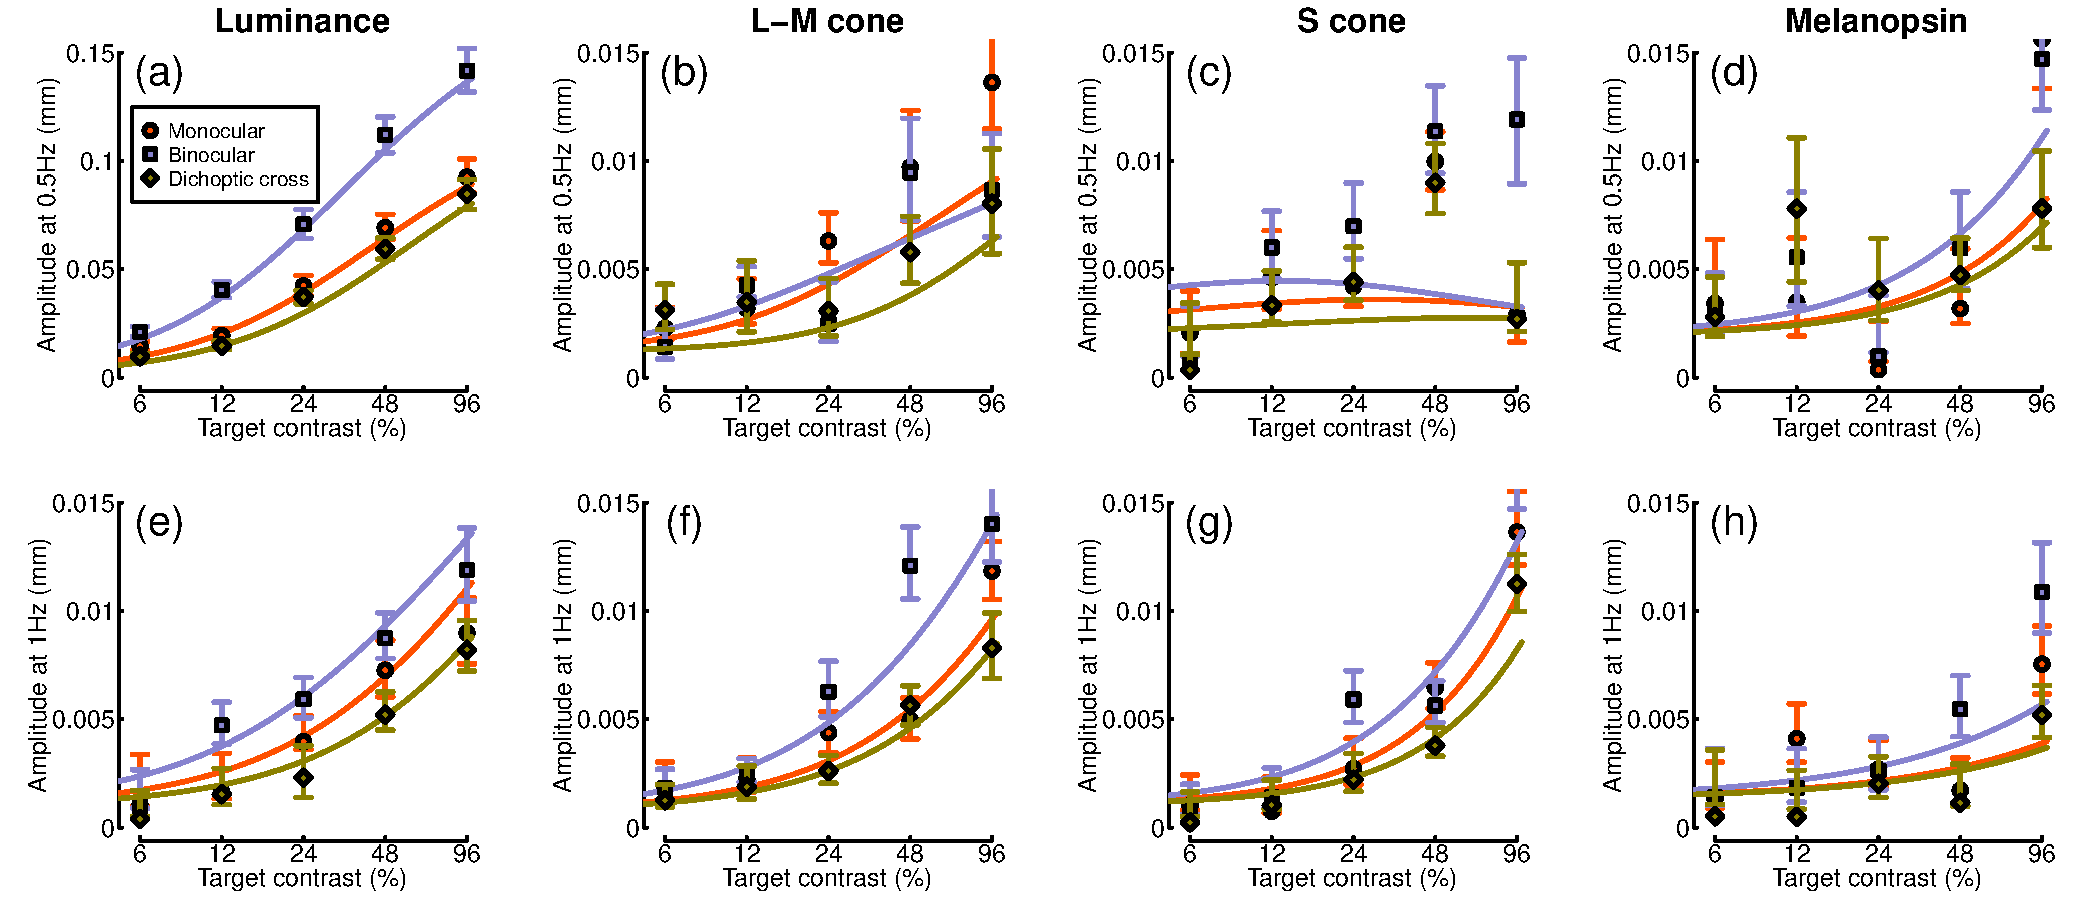
\includegraphics{Figures/CRFs} 

}

\caption{Contrast response functions for monocular (red circles), binocular (blue squares) and dichoptic (yellow diamonds) conditions, for stimulation of different pathways (columns) at the first and second harmonic frequencies (rows). Error bars indicate bootstrapped 95\% confidence intervals}\label{fig:CRFplots}
\end{figure}

In contemporary models of binocular signal combination, the amount of binocular facilitation is determined by the magnitude of interocular suppression, with strong suppression reducing facilitation (\protect\hyperlink{ref-Kingdom2015}{Kingdom and Libenson, 2015}). We can estimate the strength of interocular suppression by measuring how much monocular responses are reduced when a high contrast dichoptic mask is shown to the other eye. In our paradigm, this mask flickered at a lower frequency (0.4Hz) so that the two stimulus components remain distinct in the Fourier spectrum (e.g. \protect\hyperlink{ref-Busse2009}{Busse et al., 2009}). The yellow diamond symbols in Figure \ref{fig:CRFplots} show the target responses in this condition, and in most cases are weaker than the monocular responses (red circles). The strongest dichoptic masking is found in the first harmonic L-M condition, where we also observed the binocular suppression effect. We summarise this relationship by calculating an index for each effect, and show that the binocular facilitation effect is negatively correlated with the dichoptic masking effect (see Figure \ref{fig:suppressionfig}).

\begin{figure}

{\centering 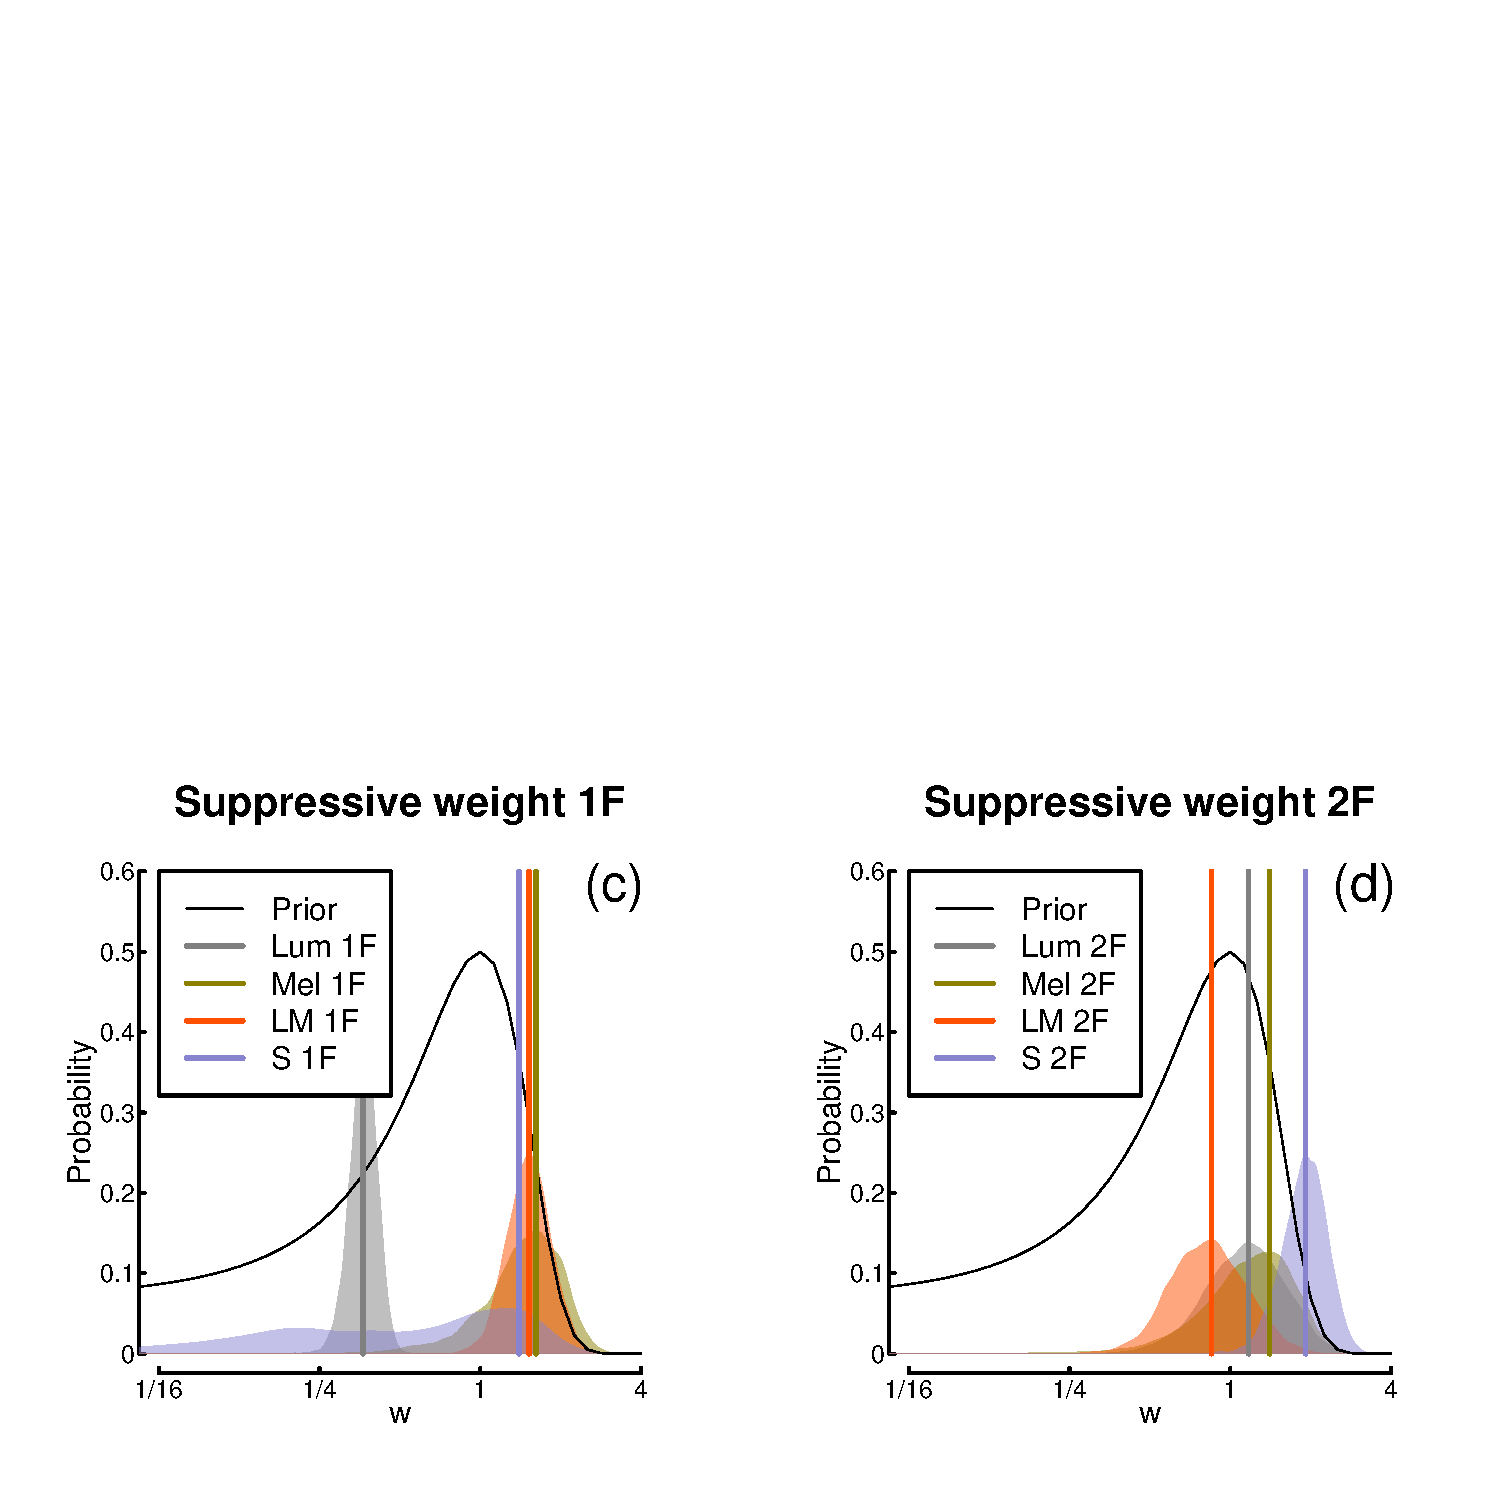
\includegraphics{Figures/suppressionfig} 

}

\caption{P.}\label{fig:suppressionfig}
\end{figure}

Next, we fitted all 8 data sets using a Bayesian hierarchical implementation of a simple binocular combination model (\protect\hyperlink{ref-Meese2006}{Meese et al., 2006}; \protect\hyperlink{ref-Segala2023}{Segala et al., 2023}). Our primary interest was to compare posterior distributions of the weight of interocular suppression, which are showin in Figure \ref{fig:suppressionfig}. Consistent with our earlier observations, at the first harmonic the strongest suppressive weight corresponds to the L-M condition, and the weakest suppression corresponds to the luminance condition (also consistent with \protect\hyperlink{ref-Segala2023}{Segala et al., 2023}). The model fits were of good quality, as shown by the curves in Figure \ref{fig:CRFplots}. Further details of fitted parameters, and model behaviour in other empirical conditions are provided in the Supplementary Materials.

Finally, we inspected the response phase of our four stimulation conditions, given previous reports that these differ across pathways (\protect\hyperlink{ref-Spitschan2014}{Spitschan et al., 2014}), and may be in antiphase for melanopsin and S-cone signals. Figure \ref{fig:phaseplots} shows the phase angles for the first (a) and second (b) harmonic frequencies for binocular stimulation (monocular stimulation produced very similar results). At the first harmonic, melanopsin and S-cone signals differed in phase by more than 90 degrees, though they were not fully in antiphase. The luminance and L-M responses were more closely in antiphase to each other, however this is likely due to our choice to modulate L+M- in the first half-cycle (corresponding to a luminance increase in the luminance condition), and L-M+ in the second half-cycle (corresponding to a luminance decrease in the luminance condition). Had we reversed this phase arrangement, we would likely have seen a close phase correspondence between the L-M and luminance conditions. Phase differences between the luminance, S-cone and melanopsin conditions are likely attributable to different lags in phototransduction at the earliest stage (i.e.~in the retina). At the second harmonic frequency (Figure \ref{fig:phaseplots}b), the luminance condition was again out of phase with the other three, and was approximately in quadrature phase with the L-M condition, and in antiphase with both the S-cone and melanopsin conditions (which were in phase with each other).

\begin{figure}

{\centering 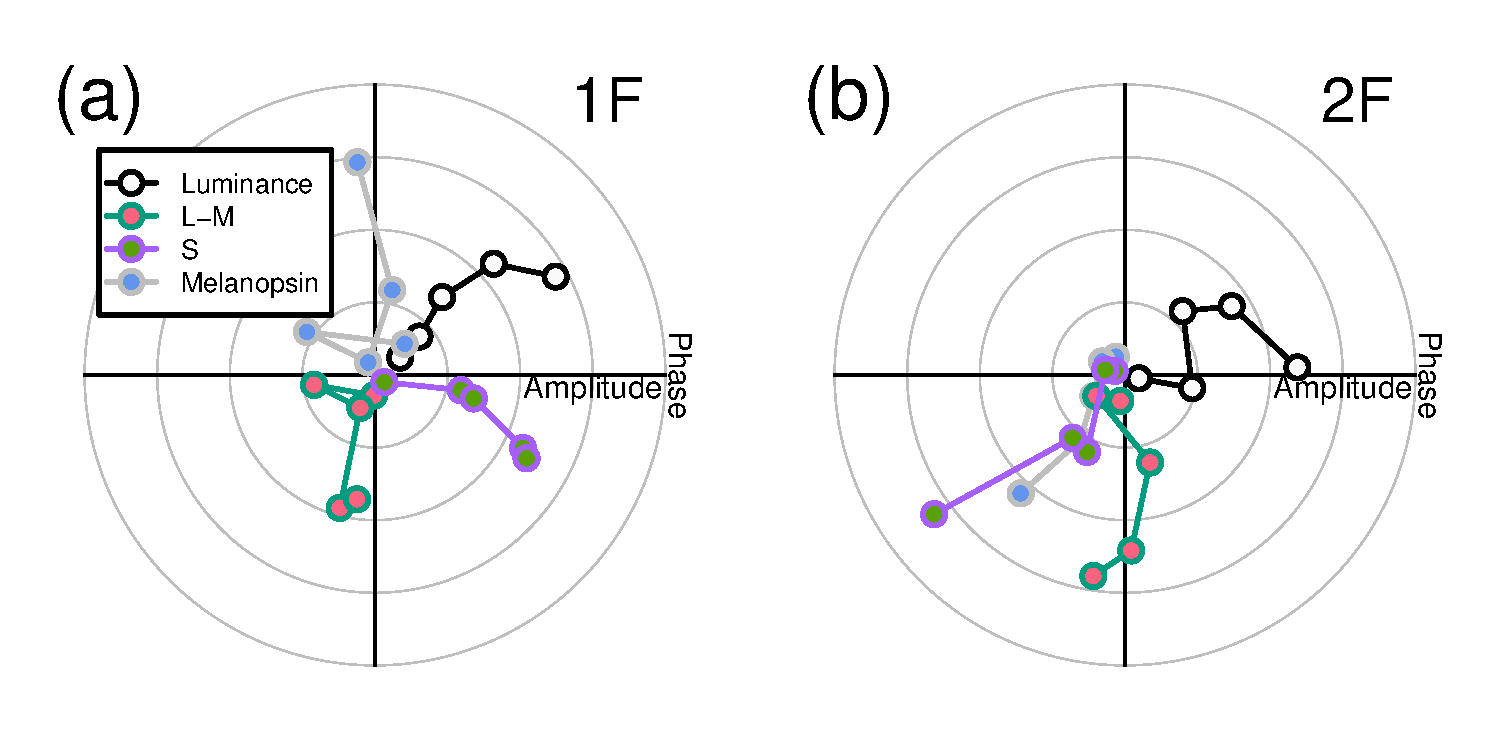
\includegraphics{Figures/phaseplots} 

}

\caption{Pupil phase plots at the first and second harmonic frequencies for the luminance, melanopsin, L-M pathway and the S-(L+M) pathway conditions Panel (a) shows the pupil response at the first harmonic frequency during binocular stimulation. Panel (b) shows the pupil response at the second harmonic frequency during binocular stimulation. In panel (a) the luminance amplitudes have been scaled down by a factor of 10 to be compared with the other conditions.}\label{fig:phaseplots}
\end{figure}

\hypertarget{discussion}{%
\section{Discussion}\label{discussion}}

We used pupillometry and silent substitution to measure monocular and binocular responses of the pupils to flickering stimuli when stimulating specific photoreceptor pathways. In our luminance experiment, we found that peripheral stimulation of the retina can elicit a pupillary response and we were also able to record a response at the second harmonic, which was not seen when we stimulated the fovea (\protect\hyperlink{ref-Segala2023}{Segala et al., 2023}). In all four experiments, we were able to record contrast response functions at both the first and the second harmonics. All experiments showed that binocular combination in the autonomic nervous system happens in a non-linear manner, with evidence of different magnitudes of interocular suppression depending on the photoreceptor pathway. This pattern of results was confirmed by a computational model, which allowed us to compare the weight of interocular suppression for each pathway. We found that, at the first harmonic frequency, the L-M pathway had a bigger suppression weight than the other pathways, while, at the second harmonic frequency, the S-(L+M) pathway had a bigger suppression weight. Finally, we looked at the pupil phases and observed different behaviours for the different pathways at the first and second harmonic frequencies. While the patterns differed between the first and second harmonics, within the same harmonic, whether the stimuli were presented monocularly or binocularly, the patterns were similar.

Our four experiments produced results that we were expecting based on our previous pupillometry findings (\protect\hyperlink{ref-Segala2023}{Segala et al., 2023}): the signals between the 2 pupils are combined non-linearly regardless of which photoreceptor pathway is being stimulated and whether the fovea or the periphery of the retina is being stimulated. We also observed responses at both the first and the second harmonic frequencies, which were expected based on previous literature (\protect\hyperlink{ref-Spitschan2014}{Spitschan et al., 2014}; \protect\hyperlink{ref-Stark1957}{Stark and Sherman, 1957}; \protect\hyperlink{ref-Verdon1988}{Verdon and Howarth, 1988}). There was, however, one aspect of our results that we were surprised to observe: the amplitude of this second harmonic response in the different photoreceptor pathways. It is true that we had already observed second harmonic responses when stimulating the periphery of the retina with achromatic luminance modulations flickering at 2 Hz (see Figure \ref{fig:appendixfig1}b), but the peak was very small when compared to the first harmonic peak, which is similar to what we observed in the luminance experiment here. On the other hand, in the melanopsin and L-M pathway experiments, the first and second harmonics are similar in amplitudes, and in the S-(L+M) pathway experiment, the peak of the second harmonic is even bigger than the peak of the first harmonic. One reason for why this might be happening may be because the driving signal is stronger when using a lower flicker frequency (indeed, pupillometry is more responsive to slow flicker frequencies of less than 1 Hz, \protect\hyperlink{ref-Spitschan2014}{Spitschan et al., 2014}) and when stimulating the periphery of the retina (we have a very clear waveform for the luminance experiment in Figure \ref{fig:pupildataLum}b). However, this explanation is not entirely satisfactory: we observed a second harmonic when stimulating the periphery using a higher flicker frequency and the pupil waveforms from the other three experiments are not as clear as the one from the luminance experiment. The presence of a second harmonic might indicate the existence of non-linearities that are not observable in the fovea: indeed, steady-state visual responses can contain activity beyond the first harmonic and these harmonics reflect non-linearities (e.g.~squaring, exponentiation, rectification) in the visual response (\protect\hyperlink{ref-Norcia2015}{Norcia et al., 2015}). Additionally, it can be the case that, when these non-linearities are strong, then the higher harmonics can have equal or even higher peaks than the first harmonic. Here, we did observe strong non-linearities in our photoreceptor pathways, as reflected by the interocular suppression weights that were output by our computational model. For the S-(L+M) pathway specifically, it seems that the higher peak of the second harmonic is a behaviour intrinsic to S cones, as this was observed previously (\protect\hyperlink{ref-Spitschan2014}{Spitschan et al., 2014}).

The pupil phases shown in Figure \ref{fig:phaseplots} give us more information about the pathways controlling the pupil response. The first thing that we notice is that the luminance and L-M pathway responses are in anti-phase. It is important to note that, for our L-M pathway stimulation, the stimulus flickered between magenta (first half of the cycle) and cyan (second half of the cycle), which means that the pupil was dilating during the magenta stimulation and then constricting during the cyan presentation. This seems to suggest that increments in magenta would correspond to decrements in brightness and increments in cyan would correspond to increments in brightness. It is possible that, if we had reversed the presentation cycle for the L-M pathway, the pupil response would have been in phase with the luminance responses. It has been recently shown that L-cone and melanopsin stimulation induce an opponent pupillary response to M- and S-cone stimulation (\protect\hyperlink{ref-Murray2018}{Murray et al., 2018}; \protect\hyperlink{ref-Woelders2018}{Woelders et al., 2018}). Our melanopsin and S-(L+M) results show a similar behaviour both for monocular and binocular responses. The L-M pathways results are desynchronised approximately in quadrature phase from the melanopsin and S-(L+M) results. These results also seem to align with what was previously found: combining L and M responses should display results that are between the opponency shown by the isolated cone stimulation. Additionally, this could explain the very strong suppression that binocular (L-M) stimulation displays compared to the monocular stimulation: if L and M produce pupil responses that are in anti-phase with each other, then combining the two together should elicit smaller responses. Finally, since the results from our experiments are not in phase, it would suggest that the photoreceptors control the pupil diameter through different pathways.

\hypertarget{conclusions}{%
\section{Conclusions}\label{conclusions}}

We have demonstrated that binocular combination of temporal flickering light in the autonomic nervous system depends on the photoreceptor pathway. We were able to elicit pupil responses by stimulating only the periphery of the retina and we were able to record contrast response functions for all photoreceptor pathways. While all pathways showed non-linear combination, they showed a variation in how the signals are combined, particularly in the weight of interocular suppression.

\hypertarget{materials-and-methods}{%
\section{Materials and methods}\label{materials-and-methods}}

\hypertarget{participants}{%
\subsection{Participants}\label{participants}}

Twenty-four participants were recruited for each of the four experiments for a total of ninety-six (68 females) adult participants, whose ages ranged from 18 to 41. All participants had normal or corrected to normal binocular vision and normal colour vision, and gave written informed consent. Our procedures were approved by the Ethics Committee of the Department of Psychology at the University of York (identification number 184).

\hypertarget{apparatus-stimuli}{%
\subsection{Apparatus \& stimuli}\label{apparatus-stimuli}}

To present synchronised stimulus modulations independently to each eye, two light engines, each with 10 independently addressable LED colour channels (SpectraTuneLAB: LEDMOTIVE Technologies, LLC, Barcelona, Spain), were integrated into a customised viewing system. The light engines were operated via a Python interface to their REST API (\protect\hyperlink{ref-Martin2022}{Martin et al., 2022}), which supports synchronous launch and playback of spectral sequences prepared in advance and stored in JSON format. When preparing the spectral sequences, the age of participants was recorded to account for the yellowing of the lenses. We calculated silent substitution solutions using the \emph{PySilSub} toolbox (\protect\hyperlink{ref-Martin2023}{Martin et al., 2023}), using linear algebra. The outputs of the two light engines (see Figure \ref{fig:spectraplots}b,c) were calibrated using an Ocean Optics Jaz spectroradiometer, which was wavelength-calibrated to an Argon lamp and intensity calibrated using a NIST-traceable light source. We used the Stockman and Sharpe (\protect\hyperlink{ref-Stockman2000}{2000}) 10-degree cone fundamentals, and estimates of melanopsin absorbance spectra from CIE S 026 (discussed in \protect\hyperlink{ref-Martin2023}{Martin et al., 2023}) to calculate \(\alpha\)-opic irradiance.

The output from the light engines was directed through liquid light guides (LLG3-8H: Thorlabs Ltd, Cambridgeshire, UK) and diffused onto semi-opaque and highly diffusive white glass discs with a diameter of 50 mm for even illumination (34-473: Edmund Optics, York, UK). The light guide gaskets were butt-coupled to the light engine diffusers with threaded adapters (SM1A9, AD3LLG: Thorlabs Ltd, Cambridgeshire, UK) and the exiting ends of the light guides were mated with 51 mm depth optical cylinders (SM2L20: Thorlabs Ltd, Cambridgeshire, UK) via appropriately threaded adapters (AD3LLG, SM2A6: Thorlabs Ltd, Cambridgeshire, UK). The stimulus diffuser discs were retained at the front end of the optical cylinders approximately 51 mm from the light source, at which distance the output beam was sufficiently dispersed to afford even illumination of the diffuser when viewed from the front. To guarantee safe illumination levels, a circular neutral-density filter with the same diameter of the white glass discs (50 mm) and an optical density of 0.6 log units was placed in the optical path between the light source and the diffusers. A small circular piece of blackout material with a diameter of approximately 8 degrees (10 mm) was positioned centrally on the front of each diffuser disc to aid as a fusion lock, as a fixation point, and to occlude the fovea.

The diffuser discs were positioned in the objective planes of the lenses of a modified VR headset (SHINECON SC-G01, Dongguan Shinecon Industrial Co.~Ltd., Guangdong, China), which was used by the participants to view the stimuli. The stimuli were two discs of flickering light with a diameter of approximately 30 degrees, which were fused together into a cyclopean percept resembling a donut-shaped ring of light, similar to that used in other studies (e.g., \protect\hyperlink{ref-Barrionuevo2016}{Barrionuevo and Cao, 2016}; \protect\hyperlink{ref-Murray2018}{Murray et al., 2018}; \protect\hyperlink{ref-Spitschan2014}{Spitschan et al., 2014}; \protect\hyperlink{ref-Zele2018}{Zele et al., 2018}). The VR headset modifications allowed for small adjustments to account for individual differences in interpupillary distance and focal length. The use of this set up allowed us to modulate the stimuli in three different ocular configurations, similar to the ones we used in our previous study (\protect\hyperlink{ref-Segala2023}{Segala et al., 2023}): monocular, binocular and dichoptic. In the monocular configuration, the unstimulated eye still saw a non-flickering disc of mean luminance. A schematic of the stimulation system is shown in Figure \ref{fig:spectraplots}a. Pupillometry data were collected using a binocular Pupil Core eye-tracker headset (Pupil Labs GmbH, Berlin, Germany, \protect\hyperlink{ref-Kassner2014}{Kassner et al., 2014}) running at 120 Hz, and the signals were recorded with the Pupil Capture software.

Our previous study (\protect\hyperlink{ref-Segala2023}{Segala et al., 2023}) used a temporal frequency of 2Hz for foveal luminance flicker, and recorded EEG data simultaneously with pupillometry. Initial pilot experiments indicated that this frequency was too high to elicit measurable responses when stimulating individual photoreceptor pathways. For all experiments, we therefore used a primary flicker frequency of 0.5Hz, as previous literature showed that it was slow enough to elicit a pupil response from all photoreceptor classes (\protect\hyperlink{ref-Spitschan2014}{Spitschan et al., 2014}). We also focussed on only recording pupillometry data as this frequency would be well below the minimum threshold to elicit steady-state EEG responses (\protect\hyperlink{ref-Norcia2015}{Norcia et al., 2015}).

For all experiments, sinusoidal temporal modulations were presented against the same background spectrum (matched between the eyes), which was used to achieve silent substitution in the three photoreceptor modulation experiments. The background spectra were defined by setting all channels to half maximum output for the brighter of the two devices (STLab 1, left eye) and then using the STLab 1/STLab 2 calibration ratio to find the equivalent settings for the companion device (STLab 2, right eye). The background spectrum illuminance was approximately 74 lux, or 62 cd/m\(^2\). The spectral power distributions and \(\alpha\)-opic irradiances of the background spectra for both eyes are shown in Figure \ref{fig:spectraplots}c-d.

In the luminance experiment, the stimulus intensity was increased and decreased relative to the background, which we expected to modulate all photoreceptor classes (see Figure \ref{fig:spectraplots}e,i). In the L-M cone modulation experiment, we used silent substution to increase the L-cone activity, and simultaneously decrease the M-cone activity, during the first half-cycle of the sine wave. In the second half-cycle the polarity of the modulation reversed (see Figure \ref{fig:spectraplots}f,j). The maximum available L-M contrast was approximately 10\%. In the S-cone modulation experiment, we increased and decreased S-cone-directed signals, whilst keeping activity in the other photoreceptors constant (see Figure \ref{fig:spectraplots}g,k). Our system allowed a maximum contrast of 45\%. Finally, in the melanopsin experiment, we modulated the activity of the melanopsin-containing intrinsically photoreceptive retinal ganglion cells, whilst keeping cone activity constant (see Figure \ref{fig:spectraplots}h,l). The maximum available melanopsin contrast was 22\%. We assume that the activity of rods was constant at the high background luminance intensity used here, and so did not attempt to silence rod activity in any condition, as this would have greatly reduced the available dynamic range. Splatter on nominally silenced photoreceptors was very small (see Figure \ref{fig:spectraplots}j-l), well below the levels that would be expected to generate measureable pupil modulations.

\hypertarget{procedure}{%
\subsection{Procedure}\label{procedure}}

Before the start of each experiment, participants adjusted the objective planes of the lenses with the help of the experimenter until the stimulus was in focus and they perceived the two pieces of blackout material as one fused disc. Pupil responses to binocular temporal contrast modulations were examined in a factorial design that combined six ocular conditions and five temporal contrast levels (6, 12, 24, 48 and 96\%) of the available dynamic range. This design, similar to that used in our previous studies (\protect\hyperlink{ref-Baker2020}{Baker et al., 2020}; \protect\hyperlink{ref-Baker2017}{Baker and Wade, 2017}; \protect\hyperlink{ref-Segala2023}{Segala et al., 2023}), was applied in four separate experiments, each with a different mode of photoreceptor stimulation. In the first three conditions, the discs flickered at 0.5 Hz, in either a monocular, binocular or dichoptic arrangement. In the dichoptic condition the non-target eye saw a flickering fixed contrast of 48\% of the available dynamic range. In the remaining three conditions (the cross-frequency conditions) one eye's disc flickered at 0.4 Hz, and the other eye's disc flickered at 0.5 Hz. We also tested monocular responses at 0.4 Hz, as well as binocular (one eye sees each frequency at the target contrast) and dichoptic (target stimulus flickering at 0.5 Hz, mask contrast of 48\% at 0.4 Hz in the other eye) arrangements. We counterbalanced presentation of the target stimulus across the left and right eyes.

The experiments were conducted in a windowless room, in which the only source of light was the modified VR headset. The participants sat as close as possible to the VR headset, leaving enough space for the eye-tracker to record the eyes. The experiment was carried out in a single session of around 45-60 minutes, divided into three blocks of 15-17 minutes each. In each block, there were a total of 60 trials lasting 15 seconds each (12s of stimulus presentation, followed by 3s of interstimulus interval). The participants were given no task other than look at the black fixation dot while trying to minimise their blinking during the presentation period. For all experiments other than the luminance condition, participants adapted to the mean luminance for two minutes before stimulation began.

Before the start of the L-M experiment, participants completed a luminance nulling perceptual calibration procedure in L-M cone space on an Iiyama \(\textrm{VisionMaster}^{\textrm{TM}}\) Pro 510 display (800 x 600 pixels, 60 Hz refresh rate). During the task, participants were presented with a disc flickering within the L-M cone space (between magenta and cyan). Using a trackball, participants adjusted the angle in cone space to find their subjective isoluminant point, which resulted in changing the flickering intensity of the stimulus until the amplitude of the flicker appeared to be minimised. The result was used to modify the requested contrasts during stimulus preparation so as to account for individual differences affecting perceived illuminance, principally the L:M cone ratio (\protect\hyperlink{ref-Carroll2002}{Carroll et al., 2002}; \protect\hyperlink{ref-Hofer2005}{Hofer et al., 2005}).

\hypertarget{data-analysis}{%
\subsection{Data analysis}\label{data-analysis}}

The pupillometry data were analysed using the same method we used in our previous study (\protect\hyperlink{ref-Segala2023}{Segala et al., 2023}). The data were converted from mp4 videos to a csv text file using the Pupil Player software (\protect\hyperlink{ref-Kassner2014}{Kassner et al., 2014}), which estimated pupil diameter for each eye on each frame using a 3D model of the eyeball. The individual data were then loaded into R for analysis, where a ten-second waveform for each trial in each eye was extracted (excluding the first two seconds after stimulus onset). We interpolated across any dropped or missing frames to ensure regular and continuous sampling over time. The Fourier transform was calculated for each waveform, and all repetitions of each condition were pooled across eye and then averaged. Finally, data were averaged across all participants to obtain the group results. We used coherent averaging and at each stage we excluded data points with a Mahalanobis distance exceeding \(D\) = 3 from the complex-valued mean (\protect\hyperlink{ref-Baker2021}{Baker, 2021}). For monocular stimulation, we confirmed that the consensual response was equivalent to the response in the stimulated eye.

For all experiments, we used a bootstrapping procedure with 1000 iterations to estimate standard errors across participants. All analysis and figure construction was conducted using a single R-script, available online, making this study fully computationally reproducible: \url{https://osf.io/gdvt4/}.

\hypertarget{computational-model-and-parameter-estimation}{%
\subsection{Computational model and parameter estimation}\label{computational-model-and-parameter-estimation}}

To describe our data, we chose the same model described in our previous study (\protect\hyperlink{ref-Segala2023}{Segala et al., 2023}). The model has the same general form as the first stage of the contrast gain control model proposed by Meese et al. (\protect\hyperlink{ref-Meese2006}{2006}) and omits the second stage. For the previous model that we used (\protect\hyperlink{ref-Segala2023}{Segala et al., 2023}), the exponent of the numerator and denominator had fixed values of 2 and (implicitly) 1. Here, we allow these parameters (called \emph{p} and \emph{q}) to be free, in order to permit different shapes of contrast response function, e.g.~saturating or super-saturating. The responses of the left eye and right eye channels are as follows:

\begin{equation}
\label{eq:respLchap4}
Resp_L = \frac{L^p}{Z + L^q + wR^q},
\end{equation}

\begin{equation}
\label{eq:respRchap4}
Resp_R = \frac{R^p}{Z + R^q + wL^q},
\end{equation}

\noindent where \emph{L} and \emph{R} are the contrast signals from the left and right eyes, \emph{p} and \emph{q} are exponents, \emph{Z} is a saturation constant that shifts the contrast-response function laterally, and \emph{w} is the weight of suppression from the other eye.

The responses from the two eyes are then summed binocularly:

\begin{equation}
\label{eq:respBchap4}
Resp_B = R_{max}(Resp_L + Resp_R) + k,
\end{equation}

\noindent where \emph{k} is a noise parameter, and \(R_{max}\) scales the overall response amplitude.

We performed model fitting on the normalised amplitudes to account for amplitude differences between the experiments. The models were fit using a hierarchical Bayesian framework implemented in Stan (\protect\hyperlink{ref-Carpenter2017}{Carpenter et al., 2017}). The data for each photoreceptor type and response frequency was fit separately, for a total of 8 model fits. The prior

\hypertarget{acknowledgements-and-funding-sources}{%
\section{Acknowledgements and funding sources}\label{acknowledgements-and-funding-sources}}

Supported by Biotechnology and Biological Sciences Research Council grant BB/V007580/1 awarded to DHB and ARW.

\hypertarget{references}{%
\section{References}\label{references}}

\hypertarget{refs}{}
\begin{CSLReferences}{1}{0}
\leavevmode\vadjust pre{\hypertarget{ref-Baker2021}{}}%
Baker DH. 2021. Statistical analysis of periodic data in neuroscience. \emph{Neurons, Behavior, Data analysis, and Theory} \textbf{5}. doi:\href{https://doi.org/10.51628/001c.27680}{10.51628/001c.27680}

\leavevmode\vadjust pre{\hypertarget{ref-Baker2018}{}}%
Baker DH, Lygo FA, Meese TS, Georgeson MA. 2018. Binocular summation revisited: Beyond \(\sqrt{2}\). \emph{Psychol Bull} \textbf{144}:1186--1199. doi:\href{https://doi.org/10.1037/bul0000163}{10.1037/bul0000163}

\leavevmode\vadjust pre{\hypertarget{ref-Baker2007}{}}%
Baker DH, Meese TS, Georgeson MA. 2007. Binocular interaction: Contrast matching and contrast discrimination are predicted by the same model. \emph{Spat Vis} \textbf{20}:397--413. doi:\href{https://doi.org/10.1163/156856807781503622}{10.1163/156856807781503622}

\leavevmode\vadjust pre{\hypertarget{ref-Baker2020}{}}%
Baker DH, Vilidaite G, McClarnon E, Valkova E, Bruno A, Millman RE. 2020. Binaural summation of amplitude modulation involves weak interaural suppression. \emph{Sci Rep} \textbf{10}:3560. doi:\href{https://doi.org/10.1038/s41598-020-60602-5}{10.1038/s41598-020-60602-5}

\leavevmode\vadjust pre{\hypertarget{ref-Baker2017}{}}%
Baker DH, Wade AR. 2017. Evidence for an optimal algorithm underlying signal combination in human visual cortex. \emph{Cereb Cortex} \textbf{27}:254--264. doi:\href{https://doi.org/10.1093/cercor/bhw395}{10.1093/cercor/bhw395}

\leavevmode\vadjust pre{\hypertarget{ref-Barrionuevo2016}{}}%
Barrionuevo PA, Cao D. 2016. Luminance and chromatic signals interact differently with melanopsin activation to control the pupil light response. \emph{Journal of Vision} \textbf{16(11)}:29. doi:\href{https://doi.org/10.1167/16.11.29}{10.1167/16.11.29}

\leavevmode\vadjust pre{\hypertarget{ref-Barrionuevo2018}{}}%
Barrionuevo PA, McAnany JJ, Zele AJ, Cao D. 2018. \href{https://www.frontiersin.org/articles/10.3389/fneur.2018.01140}{Non-linearities in the {Rod} and {Cone} {Photoreceptor} {Inputs} to the {Afferent} {Pupil} {Light} {Response}}. \emph{Frontiers in Neurology} \textbf{9}.

\leavevmode\vadjust pre{\hypertarget{ref-Barrionuevo2014}{}}%
Barrionuevo PA, Nicandro N, McAnany JJ, Zele AJ, Gamlin P, Cao D. 2014. Assessing rod, cone, and melanopsin contributions to human pupil flicker responses. \emph{Investigative Ophthalmology \& Visual Science} \textbf{55}:719--27. doi:\href{https://doi.org/10.1167/iovs.13-13252}{10.1167/iovs.13-13252}

\leavevmode\vadjust pre{\hypertarget{ref-Busse2009}{}}%
Busse L, Wade AR, Carandini M. 2009. Representation of concurrent stimuli by population activity in visual cortex. \emph{Neuron} \textbf{64}:931--42. doi:\href{https://doi.org/10.1016/j.neuron.2009.11.004}{10.1016/j.neuron.2009.11.004}

\leavevmode\vadjust pre{\hypertarget{ref-Campbell1965}{}}%
Campbell FW, Green DG. 1965. Monocular versus binocular visual acuity. \emph{Nature} \textbf{208}:191--2. doi:\href{https://doi.org/10.1038/208191a0}{10.1038/208191a0}

\leavevmode\vadjust pre{\hypertarget{ref-Cao2015}{}}%
Cao D, Nicandro N, Barrionuevo PA. 2015. A five-primary photostimulator suitable for studying intrinsically photosensitive retinal ganglion cell functions in humans. \emph{Journal of Vision} \textbf{15}:27. doi:\href{https://doi.org/10.1167/15.1.27}{10.1167/15.1.27}

\leavevmode\vadjust pre{\hypertarget{ref-Carpenter2017}{}}%
Carpenter B, Gelman A, Hoffman MD, Lee D, Goodrich B, Betancourt M, Brubaker MA, Guo J, Li P, Riddell A. 2017. Stan: A probabilistic programming language. \emph{J Stat Softw} \textbf{76}. doi:\href{https://doi.org/10.18637/jss.v076.i01}{10.18637/jss.v076.i01}

\leavevmode\vadjust pre{\hypertarget{ref-Carroll2002}{}}%
Carroll J, Neitz J, Neitz M. 2002. Estimates of {L}:{M} cone ratio from {ERG} flicker photometry and genetics. \emph{Journal of Vision} \textbf{2}:1. doi:\href{https://doi.org/10.1167/2.8.1}{10.1167/2.8.1}

\leavevmode\vadjust pre{\hypertarget{ref-Dacey2005}{}}%
Dacey DM, Liao H-W, Peterson BB, Robinson FR, Smith VC, Pokorny J, Yau K-W, Gamlin PD. 2005. Melanopsin-expressing ganglion cells in primate retina signal colour and irradiance and project to the {LGN}. \emph{Nature} \textbf{433}:749--754. doi:\href{https://doi.org/10.1038/nature03387}{10.1038/nature03387}

\leavevmode\vadjust pre{\hypertarget{ref-Dacey2003}{}}%
Dacey DM, Peterson BB, Robinson FR, Gamlin PD. 2003. Fireworks in the primate retina: In vitro photodynamics reveals diverse LGN-projecting ganglion cell types. \emph{Neuron} \textbf{37}:15--27. doi:\url{https://doi.org/10.1016/S0896-6273(02)01143-1}

\leavevmode\vadjust pre{\hypertarget{ref-Ding2006}{}}%
Ding J, Sperling G. 2006. A gain-control theory of binocular combination. \emph{Proc Natl Acad Sci U S A} \textbf{103}:1141--6. doi:\href{https://doi.org/10.1073/pnas.0509629103}{10.1073/pnas.0509629103}

\leavevmode\vadjust pre{\hypertarget{ref-Estevez1982}{}}%
Estévez O, Spekreijse H. 1982. The "silent substitution" method in visual research. \emph{Vision Research} \textbf{22}:681--691. doi:\href{https://doi.org/10.1016/0042-6989(82)90104-3}{10.1016/0042-6989(82)90104-3}

\leavevmode\vadjust pre{\hypertarget{ref-Gamlin2007}{}}%
Gamlin PDR, McDougal DH, Pokorny J, Smith VC, Yau K-W, Dacey DM. 2007. Human and macaque pupil responses driven by melanopsin-containing retinal ganglion cells. \emph{Vision Research} \textbf{47}:946--954. doi:\href{https://doi.org/10.1016/j.visres.2006.12.015}{10.1016/j.visres.2006.12.015}

\leavevmode\vadjust pre{\hypertarget{ref-Hofer2005}{}}%
Hofer H, Carroll J, Neitz J, Neitz M, Williams DR. 2005. Organization of the human trichromatic cone mosaic. \emph{The Journal of Neuroscience} \textbf{25}:9669--9679. doi:\href{https://doi.org/10.1523/jneurosci.2414-05.2005}{10.1523/jneurosci.2414-05.2005}

\leavevmode\vadjust pre{\hypertarget{ref-Hubel1962}{}}%
Hubel DH, Wiesel TN. 1962. Receptive fields, binocular interaction and functional architecture in the cat's visual cortex. \emph{J Physiol} \textbf{160}:106--54. doi:\href{https://doi.org/10.1113/jphysiol.1962.sp006837}{10.1113/jphysiol.1962.sp006837}

\leavevmode\vadjust pre{\hypertarget{ref-Kassner2014}{}}%
Kassner M, Patera W, Bulling A. 2014. Pupil: An open source platform for pervasive eye tracking and mobile gaze-based interaction.Proceedings of the 2014 {ACM} International Joint Conference on Pervasive and Ubiquitous Computing: Adjunct Publication. {ACM}. doi:\href{https://doi.org/10.1145/2638728.2641695}{10.1145/2638728.2641695}

\leavevmode\vadjust pre{\hypertarget{ref-Kingdom2015}{}}%
Kingdom FAA, Libenson L. 2015. Dichoptic color saturation mixture: Binocular luminance contrast promotes perceptual averaging. \emph{J Vis} \textbf{15}:2. doi:\href{https://doi.org/10.1167/15.5.2}{10.1167/15.5.2}

\leavevmode\vadjust pre{\hypertarget{ref-Legge1984}{}}%
Legge GE. 1984. Binocular contrast summation--II. Quadratic summation. \emph{Vision Res} \textbf{24}:385--94. doi:\href{https://doi.org/10.1016/0042-6989(84)90064-6}{10.1016/0042-6989(84)90064-6}

\leavevmode\vadjust pre{\hypertarget{ref-Lucas2003}{}}%
Lucas RJ, Hattar S, Takao M, Berson DM, Foster RG, Yau K-W. 2003. Diminished pupillary light reflex at high irradiances in melanopsin-knockout mice. \emph{Science} \textbf{299}:245--247. doi:\href{https://doi.org/10.1126/science.1077293}{10.1126/science.1077293}

\leavevmode\vadjust pre{\hypertarget{ref-Markwell2010}{}}%
Markwell EL, Feigl B, Zele AJ. 2010. Intrinsically photosensitive melanopsin retinal ganglion cell contributions to the pupillary light reflex and circadian rhythm. \emph{Clinical and Experimental Optometry} \textbf{93}:137--149. doi:\href{https://doi.org/10.1111/j.1444-0938.2010.00479.x}{10.1111/j.1444-0938.2010.00479.x}

\leavevmode\vadjust pre{\hypertarget{ref-Martin2023}{}}%
Martin JT, Boynton GM, Baker DH, Wade AR, Spitschan M. 2023. PySilSub: An open-source python toolbox for implementing the method of silent substitution in vision and nonvisual photoreception research. \emph{Journal of Vision} \textbf{23}:10. doi:\href{https://doi.org/10.1167/jov.23.7.10}{10.1167/jov.23.7.10}

\leavevmode\vadjust pre{\hypertarget{ref-Martin2022}{}}%
Martin JT, Pinto J, Bulte D, Spitschan M. 2022. PyPlr: A versatile, integrated system of hardware and software for researching the human pupillary light reflex. \emph{Behavior Research Methods} \textbf{54}:2720--2739. doi:\href{https://doi.org/10.3758/s13428-021-01759-3}{10.3758/s13428-021-01759-3}

\leavevmode\vadjust pre{\hypertarget{ref-Mathot2018}{}}%
Mathôt S. 2018. Pupillometry: Psychology, physiology, and function. \emph{J Cogn} \textbf{1}:16. doi:\href{https://doi.org/10.5334/joc.18}{10.5334/joc.18}

\leavevmode\vadjust pre{\hypertarget{ref-McDougal2015}{}}%
McDougal DH, Gamlin PD. 2015. Autonomic control of the eye. \emph{Comprehensive Physiology} \textbf{5}:439--473. doi:\href{https://doi.org/10.1002/cphy.c140014}{10.1002/cphy.c140014}

\leavevmode\vadjust pre{\hypertarget{ref-McDougal2010}{}}%
McDougal DH, Gamlin PD. 2010. The influence of intrinsically-photosensitive retinal ganglion cells on the spectral sensitivity and response dynamics of the human pupillary light reflex. \emph{Vision Research} \textbf{50}:72--87. doi:\href{https://doi.org/10.1016/j.visres.2009.10.012}{10.1016/j.visres.2009.10.012}

\leavevmode\vadjust pre{\hypertarget{ref-McDougal2008}{}}%
McDougal DH, Gamlin PD. 2008. Pupillary control pathways.The Senses: A Comprehensive Reference. Elsevier. pp. 521--536.

\leavevmode\vadjust pre{\hypertarget{ref-Meese2006}{}}%
Meese TS, Georgeson MA, Baker DH. 2006. Binocular contrast vision at and above threshold. \emph{Journal of Vision} \textbf{6}:1224--43. doi:\href{https://doi.org/10.1167/6.11.7}{10.1167/6.11.7}

\leavevmode\vadjust pre{\hypertarget{ref-Moradi2009}{}}%
Moradi F, Heeger DJ. 2009. Inter-ocular contrast normalization in human visual cortex. \emph{J Vis} \textbf{9}:13.1--22. doi:\href{https://doi.org/10.1167/9.3.13}{10.1167/9.3.13}

\leavevmode\vadjust pre{\hypertarget{ref-Murray2018}{}}%
Murray IJ, Kremers J, McKeefry D, Parry NRA. 2018. Paradoxical pupil responses to isolated {M}-cone increments. \emph{Journal of the Optical Society of America A} \textbf{35}:B66--B71. doi:\href{https://doi.org/10.1364/JOSAA.35.000B66}{10.1364/JOSAA.35.000B66}

\leavevmode\vadjust pre{\hypertarget{ref-Norcia2015}{}}%
Norcia AM, Appelbaum LG, Ales JM, Cottereau BR, Rossion B. 2015. The steady-state visual evoked potential in vision research: A review. \emph{Journal of Vision} \textbf{15(6)}:4. doi:\href{https://doi.org/10.1167/15.6.4}{10.1167/15.6.4}

\leavevmode\vadjust pre{\hypertarget{ref-Panda2002}{}}%
Panda S, Sato TK, Castrucci AM, Rollag MD, DeGrip WJ, Hogenesch JB, Provencio I, Kay SA. 2002. Melanopsin (Opn4) requirement for normal light-induced circadian phase shifting. \emph{Science} \textbf{298}:2213--2216. doi:\href{https://doi.org/10.1126/science.1076848}{10.1126/science.1076848}

\leavevmode\vadjust pre{\hypertarget{ref-Provencio2000}{}}%
Provencio I, Rodriguez IR, Jiang G, Hayes WP, Moreira EF, Rollag MD. 2000. A {Novel} {Human} {Opsin} in the {Inner} {Retina}. \emph{Journal of Neuroscience} \textbf{20}:600--605. doi:\href{https://doi.org/10.1523/JNEUROSCI.20-02-00600.2000}{10.1523/JNEUROSCI.20-02-00600.2000}

\leavevmode\vadjust pre{\hypertarget{ref-Ruby2002}{}}%
Ruby NF, Brennan TJ, Xie X, Cao V, Franken P, Heller HC, O'Hara BF. 2002. Role of melanopsin in circadian responses to light. \emph{Science} \textbf{298}:2211--2213. doi:\href{https://doi.org/10.1126/science.1076701}{10.1126/science.1076701}

\leavevmode\vadjust pre{\hypertarget{ref-Segala2023}{}}%
Segala FG, Bruno A, Martin JT, Aung MT, Wade AR, Baker DH. 2023. Different rules for binocular combination of luminance flicker in cortical and subcortical pathways. \emph{eLife} \textbf{12}. doi:\href{https://doi.org/10.7554/elife.87048}{10.7554/elife.87048}

\leavevmode\vadjust pre{\hypertarget{ref-Shapiro1996}{}}%
Shapiro AG, Pokorny J, Smith VC. 1996. Cone{\textendash}rod receptor spaces with illustrations that use {CRT} phosphor and light-emitting-diode spectra. \emph{Journal of the Optical Society of America A} \textbf{13}:2319. doi:\href{https://doi.org/10.1364/josaa.13.002319}{10.1364/josaa.13.002319}

\leavevmode\vadjust pre{\hypertarget{ref-Spitschan2019}{}}%
Spitschan M. 2019. Photoreceptor inputs to pupil control. \emph{Journal of Vision} \textbf{19}:5. doi:\href{https://doi.org/10.1167/19.9.5}{10.1167/19.9.5}

\leavevmode\vadjust pre{\hypertarget{ref-Spitschan2014}{}}%
Spitschan M, Jain S, Brainard DH, Aguirre GK. 2014. Opponent melanopsin and s-cone signals in the human pupillary light response. \emph{Proceedings of the National Academy of Sciences} \textbf{111}:15568--15572. doi:\href{https://doi.org/10.1073/pnas.1400942111}{10.1073/pnas.1400942111}

\leavevmode\vadjust pre{\hypertarget{ref-Spitschan2018}{}}%
Spitschan M, Woelders T. 2018. \href{https://www.frontiersin.org/articles/10.3389/fneur.2018.00941}{The {Method} of {Silent} {Substitution} for {Examining} {Melanopsin} {Contributions} to {Pupil} {Control}}. \emph{Frontiers in Neurology} \textbf{9}.

\leavevmode\vadjust pre{\hypertarget{ref-Stark1957}{}}%
Stark L, Sherman PM. 1957. A servoanalytic study of consensual pupil reflex to light. \emph{Journal of Neurophysiology} \textbf{20}:17--26. doi:\href{https://doi.org/10.1152/jn.1957.20.1.17}{10.1152/jn.1957.20.1.17}

\leavevmode\vadjust pre{\hypertarget{ref-Stockman2000}{}}%
Stockman A, Sharpe LT. 2000. The spectral sensitivities of the middle- and long-wavelength-sensitive cones derived from measurements in observers of known genotype. \emph{Vision Res} \textbf{40}:1711--37. doi:\href{https://doi.org/10.1016/s0042-6989(00)00021-3}{10.1016/s0042-6989(00)00021-3}

\leavevmode\vadjust pre{\hypertarget{ref-Verdon1988}{}}%
Verdon W, Howarth PA. 1988. The pupil's response to short wavelength cone stimulation. \emph{Vision research} \textbf{28}:1119--1128. doi:\href{https://doi.org/10.1016/0042-6989(88)90138-1}{10.1016/0042-6989(88)90138-1}

\leavevmode\vadjust pre{\hypertarget{ref-Wang2015}{}}%
Wang C-A, Munoz DP. 2015. A circuit for pupil orienting responses: Implications for cognitive modulation of pupil size. \emph{Curr Opin Neurobiol} \textbf{33}:134--40. doi:\href{https://doi.org/10.1016/j.conb.2015.03.018}{10.1016/j.conb.2015.03.018}

\leavevmode\vadjust pre{\hypertarget{ref-Woelders2018}{}}%
Woelders T, Leenheers T, Gordijn MCM, Hut RA, Beersma DGM, Wams EJ. 2018. Melanopsin- and {L}-cone--induced pupil constriction is inhibited by {S}- and {M}-cones in humans. \emph{Proceedings of the National Academy of Sciences} \textbf{115}:792--797. doi:\href{https://doi.org/10.1073/pnas.1716281115}{10.1073/pnas.1716281115}

\leavevmode\vadjust pre{\hypertarget{ref-Wyatt1981}{}}%
Wyatt HJ, Musselman JF. 1981. Pupillary light reflex in humans: Evidence for an unbalanced pathway from nasal retina, and for signal cancellation in brainstem. \emph{Vision Res} \textbf{21}:513--25. doi:\href{https://doi.org/10.1016/0042-6989(81)90097-3}{10.1016/0042-6989(81)90097-3}

\leavevmode\vadjust pre{\hypertarget{ref-Zele2018}{}}%
Zele AJ, Feigl B, Adhikari P, Maynard ML, Cao D. 2018. Melanopsin photoreception contributes to human visual detection, temporal and colour processing. \emph{Scientific Reports} \textbf{8}. doi:\href{https://doi.org/10.1038/s41598-018-22197-w}{10.1038/s41598-018-22197-w}

\end{CSLReferences}

\hypertarget{supplementary-materials}{%
\section{Supplementary Materials}\label{supplementary-materials}}

\begin{table}

\caption{\label{tab:paramtable1F}Summary of median parameter values at the first harmonic frequency.}
\centering
\begin{tabular}[t]{l|c|c|c|c|c|c}
\hline
Experiment & Z & k & w & p & q & Rmax\\
\hline
Luminance 1F & 96.61 & 0 & 0.37 & 1.34 & 1.28 & 0.08258\\
\hline
Melanopsin 1F & 72.80 & 0 & 1.62 & 1.18 & 0.64 & 0.00259\\
\hline
L-M 1F & 62.89 & 0 & 1.52 & 1.54 & 1.28 & 0.00287\\
\hline
S 1F & 61.56 & 0 & 1.40 & 0.41 & 1.08 & 0.04916\\
\hline
\end{tabular}
\end{table}

\begin{table}

\caption{\label{tab:paramtable2F}Summary of median parameter values at the second harmonic frequency.}
\centering
\begin{tabular}[t]{l|c|c|c|c|c|c}
\hline
Experiment & Z & k & w & p & q & Rmax\\
\hline
Luminance 2F & 63.38 & 0 & 1.17 & 1.17 & 0.94 & 0.00652\\
\hline
Melanopsin 2F & 68.76 & 0 & 1.40 & 0.88 & 0.50 & 0.00368\\
\hline
L-M 2F & 74.12 & 0 & 0.85 & 1.19 & 0.85 & 0.00472\\
\hline
S 2F & 77.31 & 0 & 1.91 & 1.36 & 0.77 & 0.00211\\
\hline
\end{tabular}
\end{table}

\end{document}
